\chapter{Servicios y herramientas}\label{S:tema_2}
Una vez resuelto los temas propiamente físicos, es necesario evaluar las diferentes posibilidades, softwares y estrategias para permitir realizar un trabajo virtualmente. Este tema muestra los diferentes puntos de interés a la hora de generar una nube y sus diversas herramientas necesarias para el día a día.

\section{Software, hardware y gestión.}
En el Anexo \ref{S:decisiones_software} se especifica el razonamiento tanto de las licencias como del tipo de software base que se utiliza en esta oficina virtual. 

El precepto es el uso de \textbf{Software libre, auto gestionado}, generalmente basado en versiones \textbf{LTS(Long Time Support) soportadas por comunidades} que dependiendo de un análisis coste/precio se auto gestiona o externaliza parcialmente.

Por ello aunque el 98\% de la utilidades y necesidades pueden ser cubiertas por software libre desde el SO (Sistema Operativo) linux, tareas ofimática y especialmente en desarrollo de software, se entiende que una licencia retail tanto de windows, como programas genéricos de ofimática puede no superar los 3-10€ siendo permanentes y fácilmente asequibles, especialmente cuando hablamos de pc/laptop desktop y no de servidores. 


Respecto a que auto gestionar y que externalizar, adoptaremos un enfoque puramente económico, minimizando los costes en base a nuestro conocimiento técnico. Por ello la principal externalización son el dominio y servidor de correo, junto a uno/dos VPS (virtual private server), como punto externo de conectividad para aplicaciones esenciales véase anexo \ref{S:anexo_mvp}, donde también se detalla el aprovisionamiento y securización anexo \ref{S:setup_abastecimiento}.

\begin{table}[!ht]
    \centering
    \begin{tabular}{|p{4cm}|p{5cm}|p{5cm}|}
    \hline
        \textbf{Requisito} & \textbf{Caso seleccionado} & \textbf{Coste} \\ \hline
        Hardware cloud base & VPS (2 cpu, 2GB/44G ram, 40 GB disk, red  250/500 Mbps) & 4-6 € / mes (dependiente de promoción) \cite{c_vps_ovh} \\ \hline
        Hardware cloud productos & VPS (2/3 cpu, 4GB ram, 80 GB disk, red  500 Mbps) & 8-12 € / mes (dependiente de promoción) \cite{c_vps_time4vps} \\ \hline
        Hardware Desarrollo & power hardware wake up on demand ( localhost ) & 20-40 € / mes coste eléctrico \\ \hline
        S.O (base) server & Linux LTS: Debian, Alma o Rocky & 0€ LTS community supported \\ \hline
        Cloud platform & Ansible \& docker \& docker-compose/swarm  & 0€ LTS community supported \\ \hline
        Services & Principalmente servicios auto alojados mediante dockerizacion & 0€ community supported \\ \hline
    \end{tabular}
\end{table}

\section{Ansible}
Ansible\cite{c_ansible} es uno de los software más utilizados actualmente como herramienta devops,  y es la principal herramienta de automatización de este trabajo. Ansible es un software de aprovisionamiento y orquestación, es decir, permite gestionar configuraciones y tareas orientadas a estado de una manera simple y centralizada.

La herramienta utiliza SSH para comunicarse desde un nodo central, utiliza YML como lenguaje descriptivo y JSON como salida. Permite usar una gran variedad de módulos para realizar tareas simples.
\begin{figure}[!htb]
\begin{center}
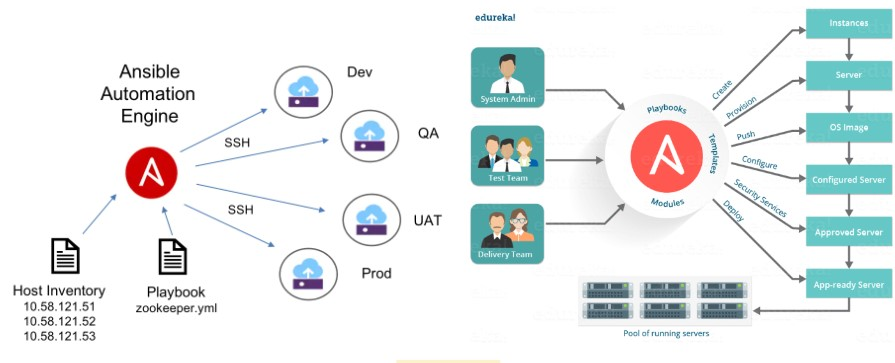
\includegraphics[width=1\textwidth]{./figuras/ansible_diagram.jpg}
\caption{Ansible diagrama funcionamiento\cite{i_ansible_1}\cite{i_ansible_2}.}
\label{F:ansible_diagram}
\end{center}
\end{figure}
El objetivo de la herramienta es generar grupos o jerarquías de servidores a los que conectarse vía SSH con los credenciales apropiados. Nótese que no es necesario de ningún software previo en dichos servidores únicamente un servicio SSH con la apropiada credencial de login.
\begin{figure}[!htb]
\begin{center}
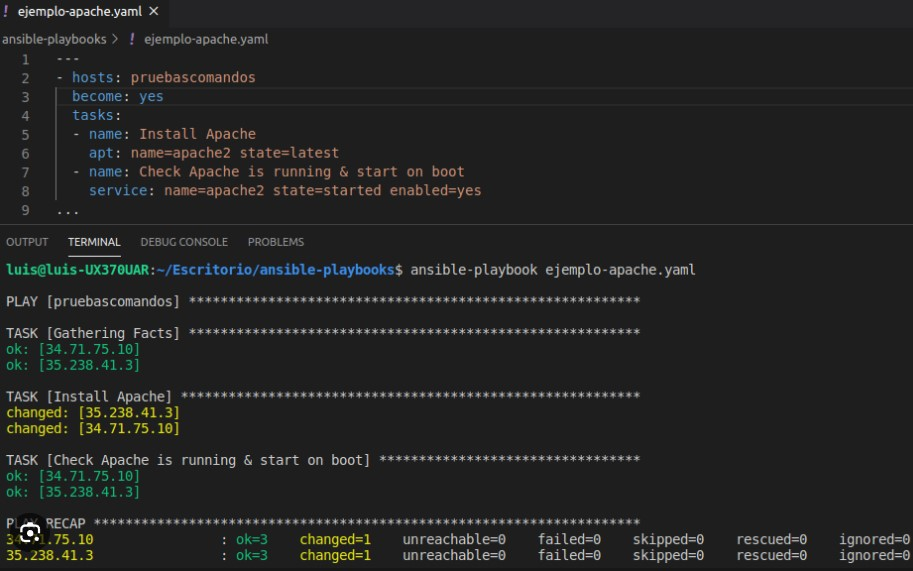
\includegraphics[width=0.9\textwidth]{./figuras/ejemplo_ansible.jpg}
\caption{Ansible ejemplo de ejecución desde proyecto VScode .}
\label{F:ejemplo_ansible}
\end{center}
\end{figure}
Una vez conectado ejecuta el comando o las tareas asociadas al script de ejecución (copiar configuraciones, ejecutar comandos, verificar estados). Estas tareas están sujetas a estado, es decir, el YML de la tarea define el estado final que se desea y el script chequea si se cumple o sino ejecuta la tarea para obtenerlo. Las tareas se ejecutan por grupo y/o tag y la ejecución se produce en paralelo en todas las máquinas.

El resultado final es que tras la ejecución del script, recibimos un output coloreado no solo con las descripción de las tareas verificadas, ejecutas  y resultado de las mismas sino con la posibilidad de acceso a un log detallado en formato json (véase fig.\ref{F:ejemplo_ansible}).

El verdadero poder de los módulos de Ansible reside en su gran abanico de opciones y softwares soportados. Permitiendo gestionar host virtualizadores o API de proveedores para crear máquinas, dispositivos de red. Ejecutar o acceder la casi totalidad de las funciones de linux y windows server. Configuración y ejecución de software de amplio uso como docker\cite{c_docker}, kubernetes\cite{c_kubernetes}, git\cite{c_git}, npm, gestores de repositorios o librerías, y la retroalimentación del output de ciertas tareas para la designación de tag o grupo de la máquina ejecutora o como input condicional para otras tareas.

Finalmente Ansible también permite la agrupación de las tareas y ficheros relacionados como rol en una estructura jerárquica de ficheros. Por lo tanto, automatizar una tarea como 'rol'. Esta estructura facilita su puesta en marcha, su actualización y su publicación en Ansible Galaxy (repositorio de rols de ansible), o lo que es lo mismo re-utilizar la gran cantidad de publicaciones de rol, evitando tener que crear un trabajo desde cero o tener acceso a innumerables ejemplos reales.

Debido al acoplamiento del caso real (Elenkar) y la sensibilidad de ciertos datos, sensibles desde el punto de vista de seguridad hacia futuros ataques, solo se han desvelado parcialmente las partes mas genéricas de dichos script, véase anexo \ref{S:ansible_ejemplo} como ejemplos.

\section{Contenedores y Docker Service}
Cuando se necesita ejecutar una aplicación o servicio se necesitan tres cosas principales, un SO que lo soporte, las librerías externas que pueda usar el software y la configuración e instalación customizada dentro del SO que lo ejecuta.

A excepción de software auto empaquetado como el de Mac OS o aplicaciones snap, la gran mayoría de softwares utilizan librerías (dll, lib) para su funcionamiento (“reusar es de pobres, pero eficiente” ). La gestión de las librerías puede conllevar a un problema cuando múltiples aplicaciones del SO requieren de librerías que entran en conflicto, o dejan de ser soportadas tras una actualización o los requisitos de máquinas virtuales de ejecución Python, Java, Php, Node, requieren de diferentes versiones en paralelo.

La necesidad de gestionar servicios pseudo duplicados que actúan sobre un mismo puerto (apache, tomcat, node) o el uso compartido de varias aplicaciones del mismo host-web. No solo hace complejo su gestión sino vulnerable ya que afecta a todos los elementos de manera transversal. La caída del servicio base o la vulneración de seguridad de una aplicación puede exponer el resto de ejecuciones del SO al compartir sistema de archivos, procesos y memoria; y solucionar este problema por VM (Máquinas virtuales) por servicio es poco eficiente y económicamente costoso.

\begin{figure}[!htb]
\begin{center}
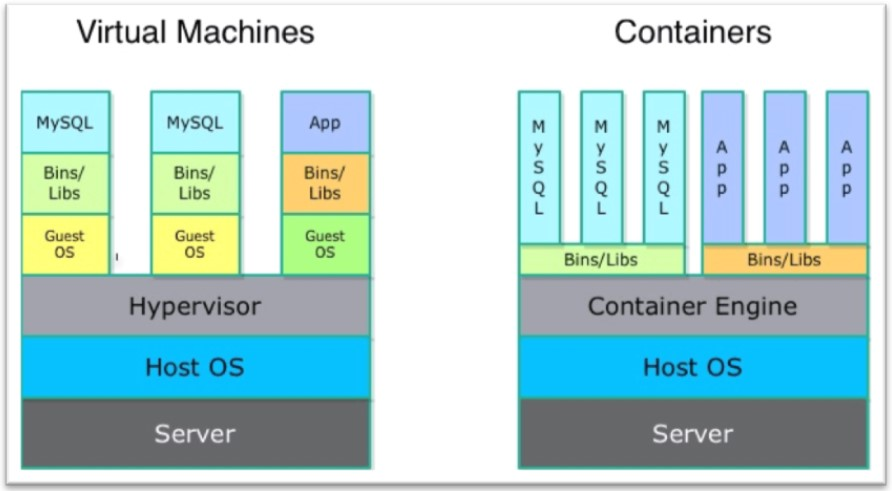
\includegraphics[width=1\textwidth]{./figuras/virtual_machine_vs_docker.jpg}
\caption{Maquina virtual vs contenedores\cite{i_containers}.}
\label{F:virtual_machine_vs_docker}
\end{center}
\end{figure}
Un contenedor, no es más que un formato estandarizado que incluye la aplicación, sus dependencias y una base de sistema operativo, para una ejecución independiente, aislada y ligera de la aplicación. A diferencia de una Virtual machine, el contenedor no emula hardware, sino que ejecuta la aplicación directamente en el kernel del sistema hospedante, sin embargo utiliza la abstracción a 'nivel de espacio de usuario' (similar chroot, cgroups y namespaces\cite{c_funcionamiento_docker}) para que el sistema de archivos, los recursos, los procesos estén aislados en el contenedor. Por otra parte, los contenedores usualmente contienen un único hilo de ejecución que es arrancado al iniciar el contenedor y cuyos cambios no son persistentes, sólo temporales mientras el contenedor está en ejecución.

Docker\cite{c_docker} es un software de código abierto usado como servicio de contenedores. Permite crear, gestionar, abstraer y automatizar el uso de contenedores permitiendo definir redes, puertos, arrancar imágenes, acceder a sus logs o mapear carpetas persistentes dentro del container.

Las imágenes de un container se crean en base a capas (como fotos del sistema de archivos), de tal manera que múltiples imágenes de aplicaciones diferentes pueden compartir capas. Si tengo múltiples imágenes de contenedores, que ejecutan software java, pero el SO (alpine) y la máquina virtual de java son iguales únicamente las capas diferentes, dependencias y aplicación serán propias de cada container. De igual manera la diferencia entre las imágenes y los container en ejecución es una última capa temporal que contiene los cambios del contenedor durante su ejecución. Entendiendo esta propiedad; es factible ejecutar múltiples containers de una misma imagen en paralelo, es decir, permite el escalado horizontal de recursos.

Por último las imágenes se pueden almacenar en repositorios como Docker Hub, que sirven a su vez no solo para arrancar contenedores sino como base para imágenes más complejas, permitiendo desarrollar tus imágenes únicamente dependientes de la capa de aplicación y delegando en comunidades el mantenimiento de aquellos elementos que no son el focus de nuestro producto.

Las principales mejoras de usar docker son:
\begin{itemize}
    \item Aislamiento, seguridad, gestión simplificada centralizada de múltiples aplicaciones dockerizadas en una única Virtual machine / servidor.
    \item Rapidez, simplicidad y sencillez en despliegue sin necesidad de instalación.
    \item Administración del sistema, sin conocimiento previo o mantenimiento sobre la aplicación.
    \item Consistencia e Independiente de plataforma, misma ejecución en test, local o producción. Facilidad en pruebas o despliegues continuos (CI/CD).
    \item Modularidad y escalabilidad horizontal, perfecto para entornos de microservicios o ambientes distribuidos.
    \item Repetibles, replicables y versionables, permite facilitar las migraciones o flexibilizar entornos y desarrollos muy ágilmente.
\end{itemize}

Por ultimo se debe entender que con el énfasis de la automatización, muchos de nuestros servicios dockerizados necesitan acceder a información de otros servicios dockerizados, por lo que en este documento se utilizan aproximaciones de docker complejas ( dind o dood) ve ase Anexo \ref{S:docker_complex}

\section{Docker Compose, Kubernetes, Docker Swarm}
Existen múltiples orquestadores sobre docker. Un orquestador de container es una capa extra de software que interacciona con nuestro engine de contenedores. Su principal ventaja es la configuración o el acceso a una interfaz más humana que el command line del engine. 

\begin{figure}[!htb]
\begin{center}

\includegraphics[width=1\textwidth]{./figuras/docker_compose_swam_kubernates.jpg}
\caption{Docker compose, swam y kubernetes logo images\cite{i_orquestadores}.}
\label{F:docker_compose_swam_kubernates}
\end{center}
\end{figure}
Sin embargo otras tareas como la definición de relaciones entre contenedores, sincronía y monitorización también son añadidas a la propia funcionalidad del engine. El mejor ejemplo es Docker-Compose\cite{c_docker_compose}, que permite configurar fácilmente en un formato YML multiples contenedores, redes, volúmenes, condiciones y relaciones entre ellos en un único fichero, permitiendo su arranque y gestión. Docker-Compose es el orquestador utilizado en este documento debido a su facilidad y el foco de una única máquina (VPS) o servidor autocrático, que actúa de manera aislada.

Sin embargo, si fuera necesario, Docker-Swarm\cite{c_docker_swarm} es un orquestador que incluye las funcionalidades de docker-compose y genera un cluster de trabajo, permitiendo unificar múltiples máquinas con servicio docker instalada como un único cluster. Facilitando no solo las herramientas de un cluster tales como master-slave, backups y balanceo de carga, sino añadiendo más herramientas no incluidas en docker-compose, como escalado, monitorización, ingress network point y encriptaciones .

Por último Kubernetes\cite{c_kubernetes} es un framework de containers, open source creado por google, que gestiona de una manera más profunda y profesional la creación y uso de un cluster de contenedores en la nube. Aunque es mi herramienta diaria de trabajo como desarrollador de software, no será usada en este trabajo puesto añade un complejidad y trabajo adicional no necesario para el nivel de requisitos de nuestros servicios donde \textbf{no se espera una gran demanda y se tiene una restricción de recursos escasos}.

\section{Arquitectura de nuestros Servicios}
La arquitectura base de la oficina virtual se fundamenta en la conjunción de tres pilares:
\begin{figure}[!htb]
\begin{center}
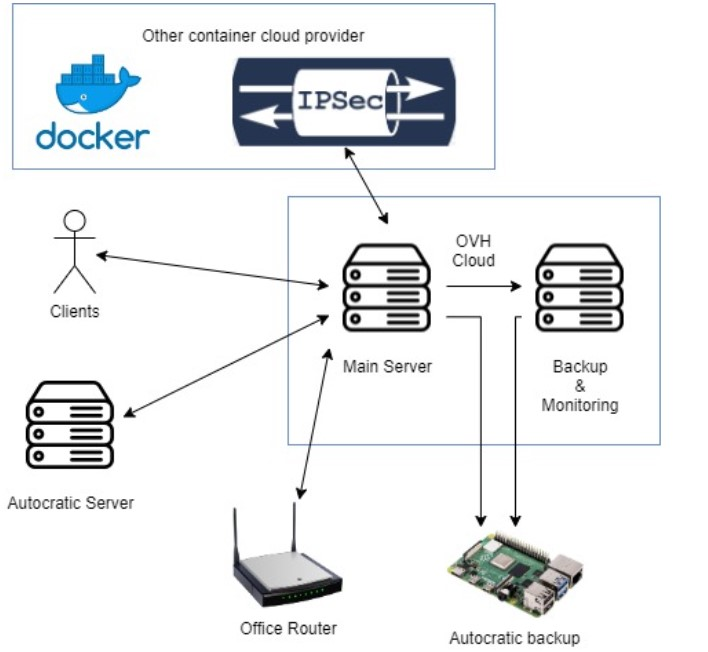
\includegraphics[width=0.75\textwidth]{./figuras/arquitectura.jpg}
\caption{Diagrama de interacción.}
\label{F:arquitectura}
\end{center}
\end{figure}
\begin{itemize}
    \item Uso de Linux LTS segurizado y automatizado que instala docker como principal servicio, minimizando y facilitando el mantenimiento de la máquina.
    \item El uso de docker y orquestadores de docker para proveer de los diferentes servicios necesarios y la interacción de los mismos.
    \item El uso de Ansible para el aprovisionamiento del servidor, la seguridad y configuración de los servicios, asi como la conetividad y configuraciones de elementos conectados al VPS por una VPN o túneles.
\end{itemize}
Los servicios públicos tales como web publica, proxy o vpn son expuestos directamente.

El servidor principal, permite conexiones reversas a los servidores-granja de producto o servidores autócratas re-enrutando el trafico. Un servidor secundario sirve como gestor de mantenimiento, monitorización y backup del principal, así como un backup autocrático en local con raspberry pi almacena el histórico de backups y configuraciones.

En todo momento, la idea es poder crecer en una nube externalizada o local, así como mantener en todo momento un control de backup. El proxy permite exponer servicios hospedados en nube externa o local a través del servidor principal VPS. La VPN permite conectar a servicios no expuestos a internet, pero si en la intranet.

Todo ello fácilmente gestionable por ansible, docker-compose que junto a los backups de configuraciones y volúmenes permiten replicar, migrar o restaurar todo en cuestión de minutos.

\section{Aprovisionamiento y Securización}
El aprovisionamiento principal es configuración, creación de grupos, permisos, eliminación de todo software innecesario del servidor, añadir docker, actualizaciones desatendidas y la autorización de claves ssh sobre un usuario administrativo de deploy.

La principal baza de seguridad de este proyecto se basa en la simplicidad, aislamiento y el uso de docker como elemento separador entre aplicaciones.

Por lo tanto, blindando del firewall y servicio SSH, la seguridad se basa en la ausencia de “accesos” y la “compartimentación”  de elementos. A excepción de los servicios públicos dockerizados y SSH no hay más servicios expuestos en la ip pública del VPS aislando y protegiendo el SO. Así mismo aquellos servicios que no requieren de ser expuestos públicamente, se utilizan internamente vía vpn - intranet.

Por lo general se puede resumir la securización del server en los siguientes conceptos:
\begin{enumerate}
    \item Purga de elementos vulnerables o no usados del sistema.
    \item Denegación de todo puerto no autorizado. Firewall ofensivo con denegación de ip.
    \item Configuración securizada de ssh. Solo permitidos non-root, vía claves asimétricas y valores default cambiados.
    \item Control con filelog, logwatch, logcheck, accounting para auditorias.
    \item Log rotate, y mecanismo de mitigación de ataques como fail2ban o denyhosts.
    \item Exponer el mínimo de servicios externamente y usar VPN para el resto.
    \item Scripts de control, sudo limitado y notificaciones de procesos de superusuarios.
    \item Usar VPN e integrar una nodo (raspberry pi o similar) con NIDS (Network Intrusion Detectors System) como prevención en redes locales interconectadas.
    \item Usar imágenes docker oficial o auto-ensambladas, que siguen buenas prácticas o escáneres de seguridad (docker hub lo incluye).
\end{enumerate}

Véase rol del Ansible de segurización \cite{c_code} y el anexo \ref{S:anexo_segurizacion} .

\section{Servicios}
En este apartado se indican los servicios seleccionados como nube MVP(Minimum Viable Product), en el anexo  \ref{S:anexo_mvp} se detallan razonamiento, posibles candidatos y una argumentación sobre cada uno de los principales servicios. En la tabla ~\ref{T:mvo_mas_diez} y  ~\ref{T:mvp_nube_seleccionado}, indican como obligatorios los marcados con un a ’*’. En el caso de que la nube se aplique a un grupo de trabajo de 10 o mas personas se incluyen los siguientes servicios:
\begin{table}[!htb]
\caption{Docker services más de 10 personas.}
\label{T:mvo_mas_diez}
\begin{tabular}{|p{2cm}|p{3cm}|p{5cm}|p{2cm}|}
\hline
\multicolumn{1}{|c|}{\textbf{Tipo de Servicio}} & \textbf{Herramienta} & \multicolumn{1}{c|}{\textbf{Detalles}} & \multicolumn{1}{c|}{\textbf{Tipo y Coste}} \\ \hline
Comunicación Interna \textgreater{}10 trabajadores & Rocket Chat\cite{c_rocket_chat} & Requiere recursos y mantenimiento continuado, es decir, servidor dedicado & Interno VPS dedicado 3-5€ / mes \\ \hline
Autenticación Centralizada & KeyCloak\cite{c_keycloak} con LDAP\cite{c_ldap} & Utilizar un LDAP que suministra información a KeyCloak y automatizar la carga de LDAP & Interno 0€ VPS principal \\ \hline
\end{tabular}%
\end{table}

\begin{table}[!htb]
\caption{Servicios docker nube MVP.}
\label{T:mvp_nube_seleccionado}
\begin{tabular}{|p{2cm}|p{3cm}|p{5cm}|p{2cm}|}
\hline
\multicolumn{1}{|c|}{\textbf{Tipo de Servicio}} & \textbf{Herramienta} & \multicolumn{1}{c|}{\textbf{Detalles}} & \multicolumn{1}{c|}{\textbf{Tipo y Coste}} \\ \hline
Correo Electrónico * & Don Dominio\cite{c_dondominio} & Externo 10 € / año 10 cuentas 3 GB o 20 € / año 15 cuentas 10 GB. & Externo 10 € / Año \\ \hline
Comunicación Externa* & Teams, Zoom, Whatsapp, Telegram & Centralizadas desde cliente Fermi. & Externa, 0€ \\ \hline
Comunicación Interna & Teams / Slack & Es un elemento excesivamente costoso, en recursos. Se usara servicio gratuito limitado. & Externa, 0€ \\ \hline
Almacenamiento* & Nextcloud\cite{c_nextcloud} & Requiere recursos, es decir, servidor VPS dedicado o via intranet a un server autocratico. & Interno 3-5€ / mes \\ \hline
Aplicación ofimática & Only Office / collabora\cite{c_colabora} & Hosteado junto a next cloud en un server dedicado. & Interno incluido nextcloud server \\ \hline
Wiki* & Bookstackapp\cite{c_bookstack} / MediaWiki\cite{c_media_wiki} & Ligero y útil para desarrollo. & Interno 0€ VPS \\ \hline
VPN* & Wire Guard\cite{c_wireguard} & Punto externo de conexiona intranet, generación de múltiples VPN. & Interno 0€ VPS \\ \hline
Repositorio de Code & Gitea\cite{c_gitea} & Si es publico en servidor VPS principal, si es privado puede estar en un server autocrático. & Interno 0€ VPS \\ \hline
CI/CD & Jenkins\cite{c_jenkins} / Drone \cite{c_drone}& Si es publico en servidor VPS principal, si es privado puede estar en un server autocratico. & Interno 0€ VPS \\ \hline
Web Service* & WordPress\cite{c_wordpress} / Static web\cite{c_hugo} & Simplemente como pagina web principal y/o blog & Interno 0€ VPS \\ \hline
Ticketing & Taiga\cite{c_taiga} & Simple y eficiente board de scrum-agile. & Interno 0€ VPS \\ \hline
\end{tabular}%
\end{table}

Es importante recordar que en las pruebas de concepto anexo \ref{S:pruebas_concepto} no se ha automatizado el proceso de configuración de interacción entre los servicios, en el caso de autenticación. 

El tuning de los plugins o las third parties, debe hacerse manualmente durante la primer arranque de la nube. Este proceso puede automatizarse pero requiere un conocimiento específico de cada servicio y tiempo dedicado excesivo, por lo que se ha priorizado la prueba de múltiples servicios y la selección del más conveniente, ya que una vez configurado apropiadamente, puede usarse el primer backup como producto pre configurado de la nube. 

Finalmente recordar que no es necesario el uso de todos los servicios, es decir, la empresa u oficina virtual debe hacer uso en función de sus necesidades, tanto en tamaño de grupo de trabajo, criterios de seguridad y monitorización etc ... deben ser coherentes con las necesidades.
\clearpage

\section{Múltiples Docker compose y limitaciones}
Para la puesta en marcha tanto de servicios externos, así como servicios no expuestos debemos de entender que muchos de ellos tiene bases de datos o servicios auxiliares, es decir por ejemplo el servicio de web puede ser un único container con todo (db,wordpress,web server, php) o puede ser múltiples container aportando cada uno su propio sub-servicio. Por lo tanto ya sea por catalogación o por simplicidad no es práctico la generación de un único docker-compose con todos los servicios. 

Lo óptimo es la definición de servicios o grupos de servicio bajo un único docker-compose, facilitando la tarea de instaurar un servicio systemD\cite{c_docker_compose_systemD} de Linux, que arranque los servicios junto con el Sistema operativo. Otro elemento útil es el uso de “Múltiples file call”\cite{c_docker_compose_multiples} en casos complejos o de elementos comunes permitiendo importar sub-ficheros yml para conformar un docker-compose final o sobre-escribir un fichero con otro \cite{c_docker_compose_override}. Par aun mayor detalle véase anexo \ref{S:docker_compose_details}.

La principal limitación de docker-compose es su aplicación en un único host, lo que limita su uso a entornos de desarrollo/testing o como nuestro caso aquellas herramientas que no requieren de una alta disponibilidad y demanda, ya que no implementa de manera nativa ningún tipo de escalado o balanceo de carga. Sin embargo si utilizamos versiones superiores a la V3, es plausible deployar directamente ficheros docker-compose en cluster de docker swarm previamente inicializados facilitando la evolución hacia un escalado horizontal de recursos.

\section{Docker Backups}
Como se ha mencionado en el anterior punto, se ha priorizado la configuración manual de plugins o interrelaciones entre los servicios, sobre la “auto-creación por script” ya que requiere de un tiempo y esfuerzo sobre dimensionado para el objetivo de este trabajo, que es tener una nube, pero no auto-configurar ágilmente.

Sin embargo sí es objetivo que esta nube se pueda construir y destruir o realizar una restauración ágilmente, es decir, se definen y configuran las relaciones entre servicios, se realiza un backup que puede ser usado como base de construcción para nuevos despliegues (siempre y cuando se mantenga la selección de servicios e interrelación). Por lo tanto la generación de backups periódicos para posibles restauraciones, así como el despliegue de backups como nuevas nubes es un elemento obligatorio.

Toda la información que los servicios desplegados contienen se fundamenta en las capas variable de los contenedores y en los volúmenes persistentes, es decir, con el apropiado backup de volúmenes, los contenedores son capaces de re-arrancar con todo apropiadamente configurado. 

Muchas veces los servicios dependen de otros servicios auxiliares tales como bases de datos, en estos casos dependiendo de si se aplicado una política de centralización en una única base de datos o en múltiples, puede hacerse el backup “por servicio” exportando sus schemas, o realizarse directamente un backup del volumen de la ddbb.

En todo caso el procedimiento siempre sigue una pauta marcada, que únicamente es influenciada por los recursos que disponemos en el VPS:
\begin{enumerate}
    \item Parada de servicios, excepto ddbb o similares.
    \item Backup de ddbb o servicios auxiliares por script.
    \item Apagado de todo servicio y realización de backup de volúmenes.
    \item Reiniciado de servicios.
\end{enumerate}


El punto crítico es la capacidad de procesado así como el espacio limitado en disco. 

Existen múltiples puntos de vista a la hora de realizar el backup usualmente se utilizan métodos de diferenciado binario con checksum (similar a git) y compresión para generar layers de cambio de las que se almacena un número máximo de veces. 

Existen software especializados también dockerizados como autorisc\cite{c_autorisc} o duplicati\cite{c_duplicati}, sin embargo el punto principal de este backup en el VPS es minimizar el uso de recursos por ello se sobreentiende que verdaderamente el backup es una sincronización en red, utilizando software como rsync\cite{c_rsync}, que sincroniza los folders de los volúmenes con un servidor remoto y es allí donde se realiza el proceso de backup propio y almacenado del último backup en un medio donde la capacidad no es un problema, ni existen limitaciones de cpu.

Entiéndase también que la realización del backup es automática-global, aunque se permita por la estructura de carpetas y subcarpetas la realización parcial de backup manualmente. 

\section{Automatizaciones y scripts}
Una vez seleccionados los servicios necesarios para nuestra nube y su prueba de concepto validada, es necesario la realización de automatizaciones para su uso diario y gestión:
\begin{itemize}
    \item Ansible y script de despliegue, son principalmente scripts de ansible que deben permitirnos un despliegue rápido desde cero de todos nuestros servicios. Dicho despliegue debe validar y llamar a script de securización y aprovisionamiento si las máquinas elegidas, si no están apropiadamente predispuestas.
    \item Apagado, encendido de la plataforma, haciendo énfasis en la automatización de muchos servicios o grupos de servicios como servicio de systemd\cite{c_systemd}, incluyendo la inicialización de los mismo al reiniciar la máquina linux  (véase anexo \ref{S:systemD} ).
    \item Cron, script o ansibles de backups, purgado de datos y chequeos de seguridad y actualización. Su principal función es verificar la seguridad y consistencia de las máquinas linux, gestionando un apagado para la realización de backups, limpieza y reinicio de la plataforma principalmente en horario nocturno (3-5 am).
    \item Validación de ecosistema, los anteriores apartados hacen referencia a máquinas exclusivamente centradas en VPS o servidores, pero es necesario una validación y gestión del cloud en todas las características añadidas, redes, conexiones vpn a otros servidores o entornos de trabajo.
\end{itemize}

\section{Legalidad}
Este apartado indica únicamente una tendencia o recomendaciones a la hora de evaluar los requisitos y riesgos legales de nuestra nube. Como ciudadanos europeos o empresas que trabajen dentro de el área económica europea, debemos tener claro 2 pilares fundamentales:
\begin{itemize}
    
    \item Cumplir la carta de derechos fundamentales de la UE y directivas o reglamentos europeas de protección de datos\cite{c_ue_rpgd}, ya que estas incluyen las leyes nacionales\cite{c_boe_rpgd} de los diferentes estados en temas de protección de datos, derechos u obligaciones en el mundo digital europeo.
    
    \item Servidores europeos o equivalentes, es decir, muchos de los requisitos necesarios se adquieren al usar un proveedor europeo con sede en Europa, o en países homologados para datos europeos. Este punto es especialmente conveniente, debido a que raramente se utilizan nubes lejanas geográficamente debido a la degradación de propiedades de red como el ping, availability, bw que degradan la conexión.
    
\end{itemize}

La recomendación como desarrollador que impera, para evitar la complejidad y el sobre esfuerzo de tratar con datos sensibles, es "\textbf{utiliza única y exclusivamente aquellos datos realmente necesarios"}, haciendo especial énfasis en evitar aquellos datos de especial sensibilidad como religión, tendencia sexual, etnia, afiliaciones políticas o sindicales, genéticos, biométricos identifica-torios, relativos a historial de salud o datos traceable.

La segunda recomendación es no vincular datos personales con otros conjuntos de datos almacenados, facilitando la eliminación de los mismos en el plazo de conservación de los datos de carácter personal.

La tercera recomendación es, segmenta, clasifica tus datos o modifícalos degradando su sensibilidad. Degradar o hacer anonimo un dato significa implica tener un dato sensible como la MAC, IP u otros identificadores que por su carácter único y identificativo es necesario. Se pueden transformar vía hash o checksum obteniendo un segundo valor que no tiene las clasificación de datos personal pero mantiene su carácter único y traceador para nuestro aplicativo.  

\subsection{Clasificación de datos e inventario}
Es importante inventariar y clasificar los datos utilizados en la nube o software. Se recomienda una clasificación a tres niveles:
\begin{enumerate}
    \item Confidencial: un dato que requiere no ser expuesto y por lo tanto no puede almacenarse en claro. Limitando el acceso al valor.
    \item Activo critico: es un dato confidencial con integridad y 'availability', es decir, permite verificar su no modificación y un procedimientos de acceso garantizado.
    \item Datos personales identificables, es un activo critico de carácter personal, por lo que incluye una clausula de tiempo de almacenamiento y eliminación el tiempo máximo legal.
\end{enumerate}

\subsection{Consentimiento y mecanismo de acceso}
Cuando obligatoriamente necesitamos un dato sensible, es muy importante que el tratamiento se base en el consentimiento del interesado, el responsable deberá ser capaz de demostrar que aquel consintió el tratamiento de sus datos personales. Por lo tanto el consentimiento debe ser inequívoco y explícito, ya que tiene la responsabilidad jurídica de demostrar que el usuario ha dado su permiso. Como ejemplo \textbf{no se puede poner pre-marcado por defecto la aceptación de política de privacidad}.

Por otra parte en todo momento existen unos procedimientos\cite{c_aedp} para atender las demandas de los clientes sobre sus derechos, y dichos procedimientos deben ser visibles, accesibles y sencillos.